\documentclass{article}
\usepackage{amsfonts, amsthm, amsmath, amssymb, mathtools, ulem, mathrsfs, physics, esint, siunitx, tikz-cd}
\usepackage{pdfpages, fullpage, color, microtype, cancel, textcomp, markdown, hyperref, graphicx}
\usepackage{enumitem}
\graphicspath{{./images/}}
\usepackage[english]{babel}
\usepackage[autostyle, english=american]{csquotes}
\MakeOuterQuote{"}
\usepackage{xparse}
\usepackage{tikz}
\usepackage{algpseudocode}

% fonts
\def\mbb#1{\mathbb{#1}}
\def\mfk#1{\mathfrak{#1}}
\def\mbf#1{\mathbf{#1}}
\def\tbf#1{\textbf{#1}}

% common bold letters
\def\bP{\mbb{P}}
\def\bC{\mbb{C}}
\def\bH{\mbb{H}}
\def\bI{\mbb{I}}
\def\bR{\mbb{R}}
\def\bQ{\mbb{Q}}
\def\bZ{\mbb{Z}}
\def\bN{\mbb{N}}

% brackets
\newcommand{\br}[1]{\left(#1\right)}
\newcommand{\sbr}[1]{\left[#1\right]}
\newcommand{\brc}[1]{\left\{#1\right\}}
\newcommand{\lbr}[1]{\left\langle#1\right\rangle}

% matrices
\newcommand{\m}[2][b]{\begin{#1matrix}#2\end{#1matrix}}
\newcommand{\arr}[3][\sbr]{#1{\begin{array}{#2}#3\end{array}}}
\DeclareMathOperator{\Span}{span}

% greek
\newcommand{\e}{\epsilon}
\newcommand{\p}{\varphi}
\renewcommand{\t}{\theta}

% misc
\NewDocumentCommand{\app}{O{x} O{\infty}}{\xrightarrow{#1\to#2}}
\newcommand{\sse}{\subseteq}
\renewcommand{\ss}{\subset}
\newcommand{\vn}{\varnothing}
\newcommand{\inv}{^{-1}}
\newcommand{\imp}{\implies}
\newcommand{\impleft}{\reflectbox{$\implies$}}
\renewcommand{\ip}[2]{\lbr{#1,#2}}
\renewcommand{\bar}{\overline}
\DeclareMathOperator{\cis}{cis}
\DeclareMathOperator{\Arg}{Arg}
\renewcommand{\d}{\partial}
\newcommand{\pf}{\tbf{Proof. }}
\renewcommand{\L}{\mathcal{L}}

% title
\title{Scientific Computing HW 7}
\author{Ryan Chen}
%\date{\today}
\setlength{\parindent}{0pt}


\begin{document}
	
\maketitle



\begin{enumerate}
	
	
	
	\item Code: \url{https://github.com/RokettoJanpu/scientific-computing-1-redux/blob/main/hw7p1.ipynb}
	
	\begin{enumerate}
		
		
		
		\item The low rank factorization is as follows. To update row $i$ of $X$, find $x_i^T$ as given in the lecture notes. To update column $j$ of $Y^T$, i.e. row $j$ of $Y$,
		\[y_j = \mathrm{argmin}_y\br{\frac12\norm{X_{\Omega^j}y - a_{\Omega^j}}_2^2 + \frac\lambda2\norm{y}_2^2}\]
		where $\Omega^j:=\brc{i:(i,j)\in\Omega}$ and $X_{\Omega^j}$ is the set of rows of $X$ with indices in $\Omega^j$, and $a_{\Omega^j}$ is the set of known entries of $A$ in column $j$.
		
		\begin{center}
			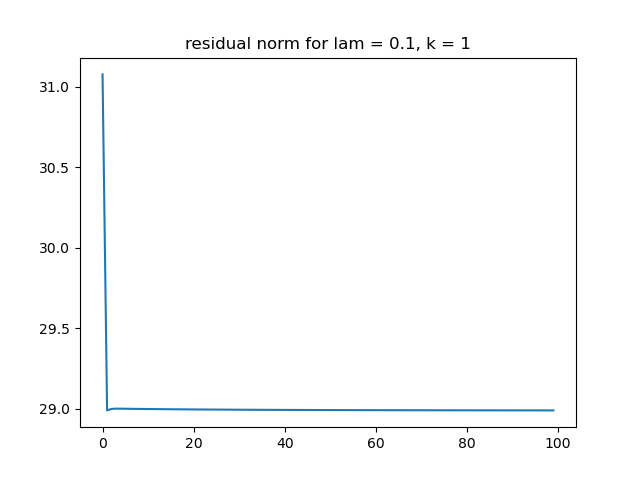
\includegraphics[scale=.3]{hw7p1 residual norm for lamcount = 1, k = 1}
			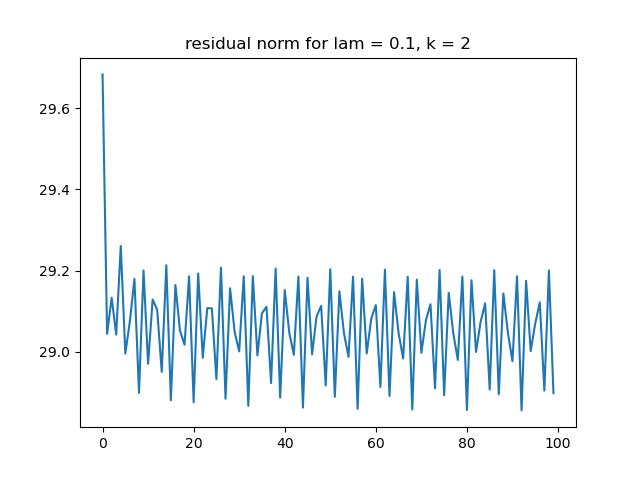
\includegraphics[scale=.3]{hw7p1 residual norm for lamcount = 1, k = 2}
			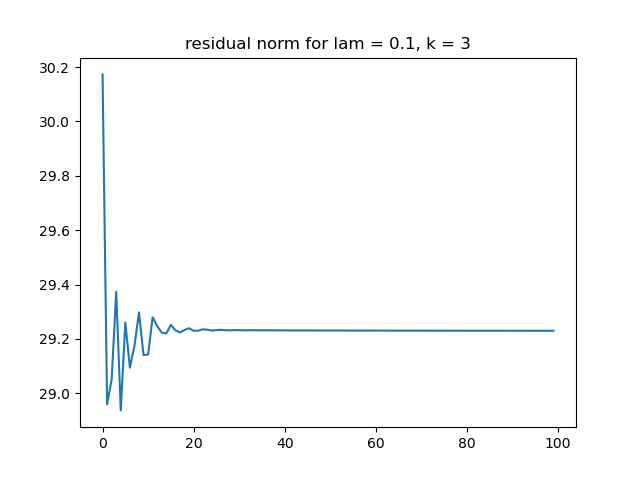
\includegraphics[scale=.3]{hw7p1 residual norm for lamcount = 1, k = 3}
			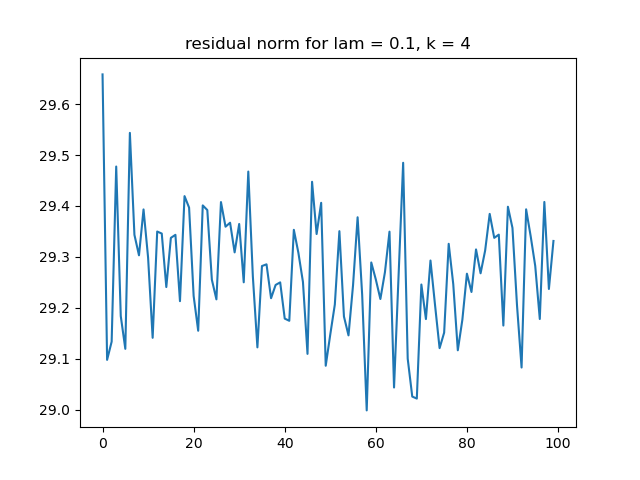
\includegraphics[scale=.3]{hw7p1 residual norm for lamcount = 1, k = 4}
			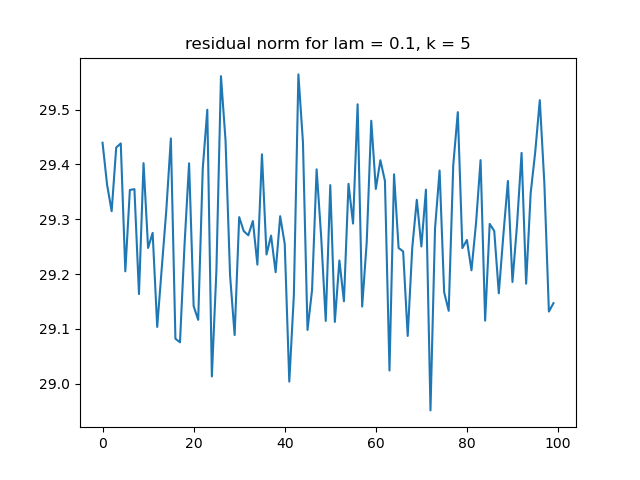
\includegraphics[scale=.3]{hw7p1 residual norm for lamcount = 1, k = 5}
			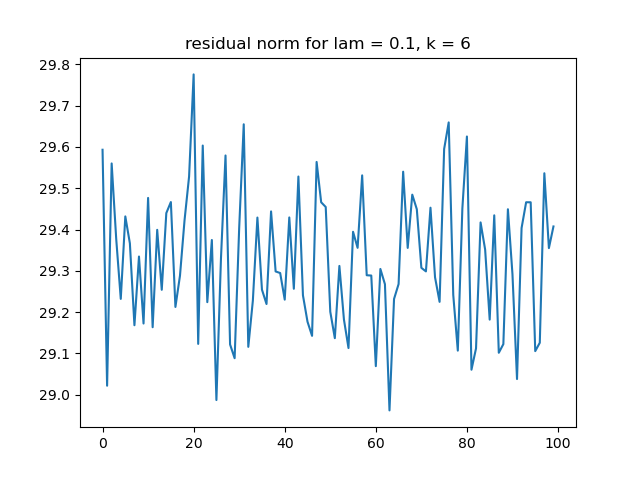
\includegraphics[scale=.3]{hw7p1 residual norm for lamcount = 1, k = 6}
			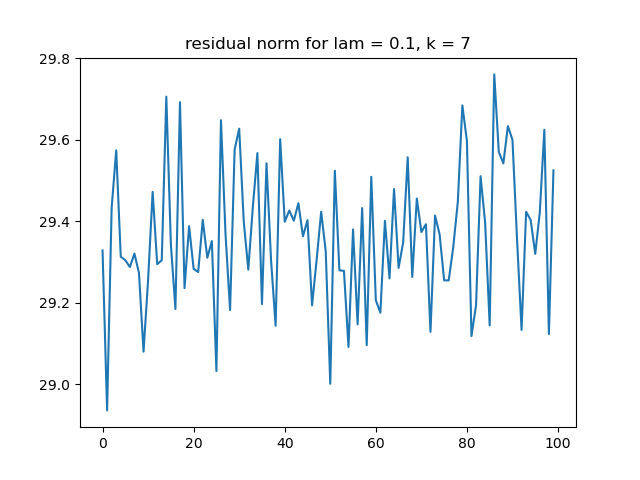
\includegraphics[scale=.3]{hw7p1 residual norm for lamcount = 1, k = 7}
			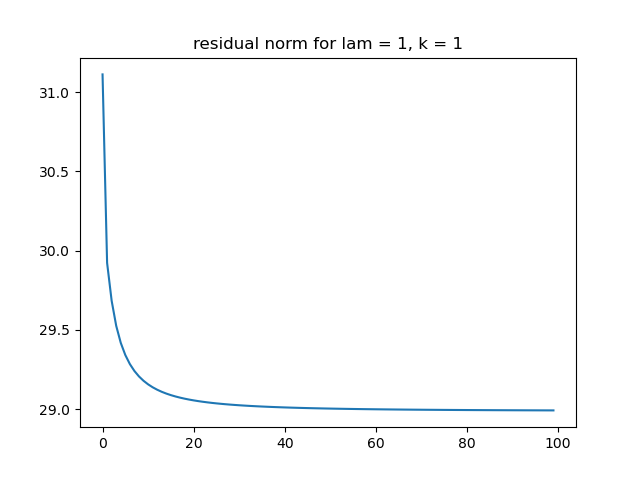
\includegraphics[scale=.3]{hw7p1 residual norm for lamcount = 2, k = 1}
			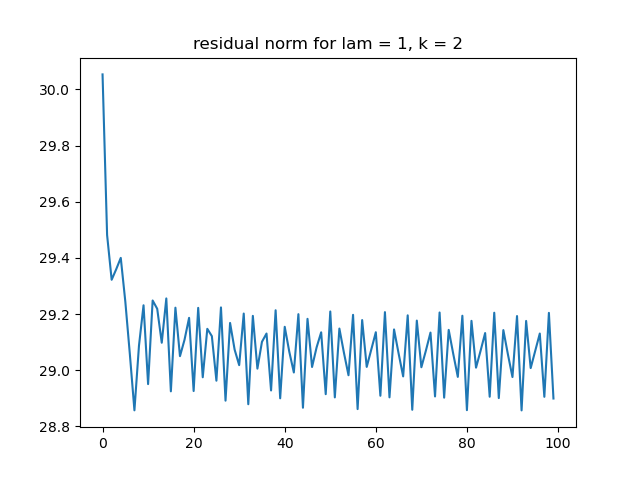
\includegraphics[scale=.3]{hw7p1 residual norm for lamcount = 2, k = 2}
			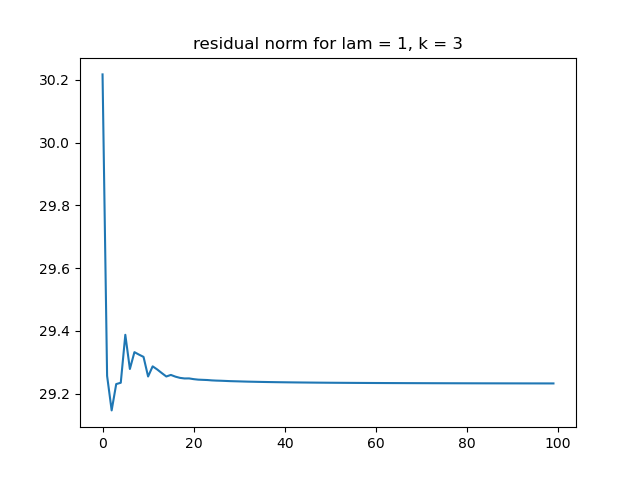
\includegraphics[scale=.3]{hw7p1 residual norm for lamcount = 2, k = 3}
			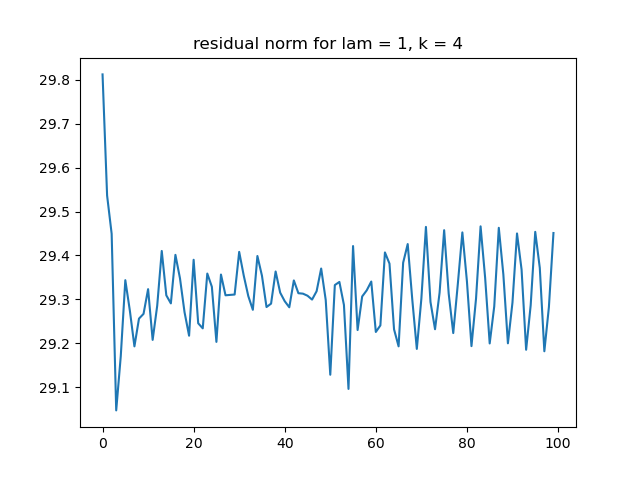
\includegraphics[scale=.3]{hw7p1 residual norm for lamcount = 2, k = 4}
			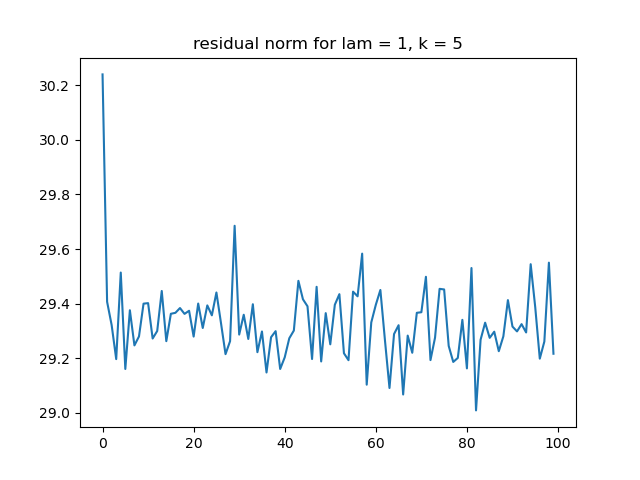
\includegraphics[scale=.3]{hw7p1 residual norm for lamcount = 2, k = 5}
			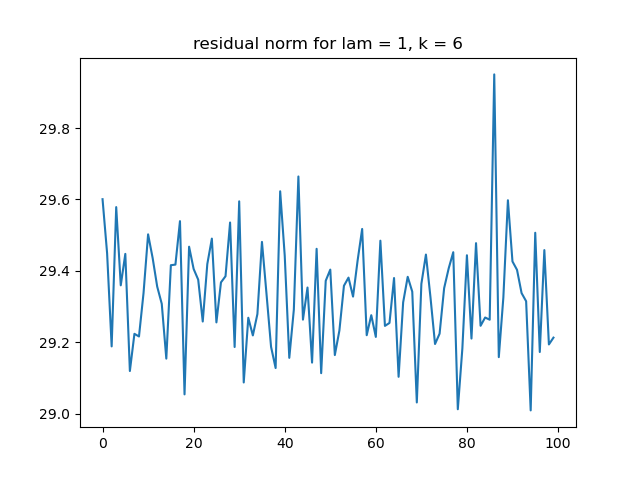
\includegraphics[scale=.3]{hw7p1 residual norm for lamcount = 2, k = 6}
			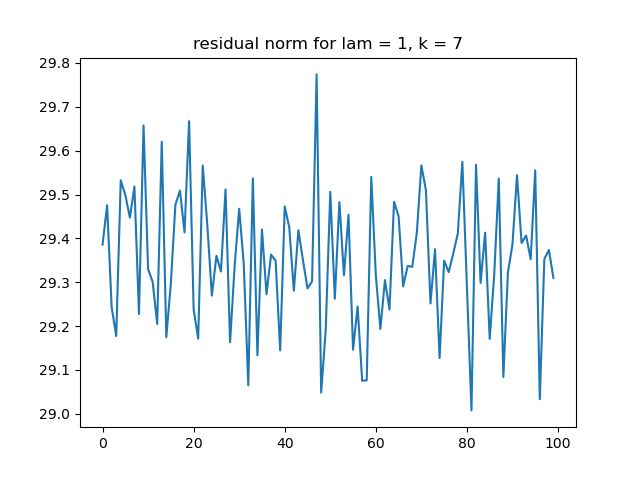
\includegraphics[scale=.3]{hw7p1 residual norm for lamcount = 2, k = 7}
			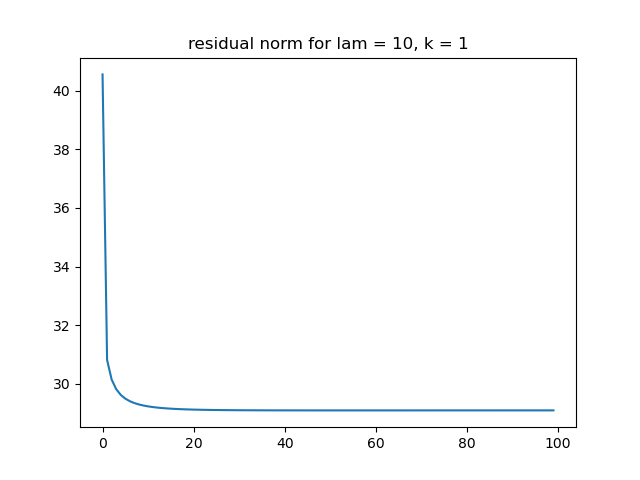
\includegraphics[scale=.3]{hw7p1 residual norm for lamcount = 3, k = 1}
			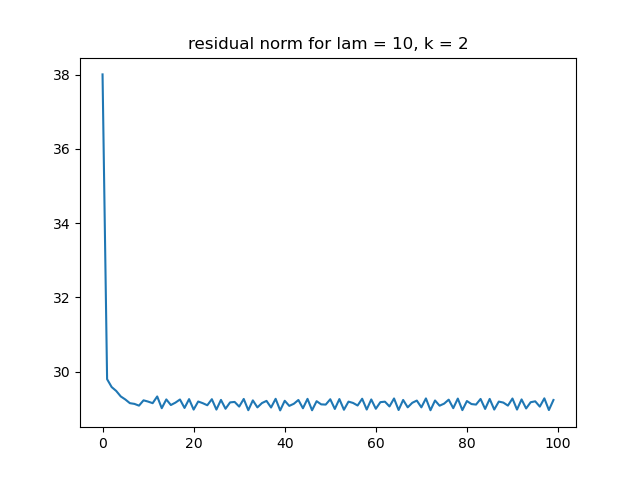
\includegraphics[scale=.3]{hw7p1 residual norm for lamcount = 3, k = 2}
			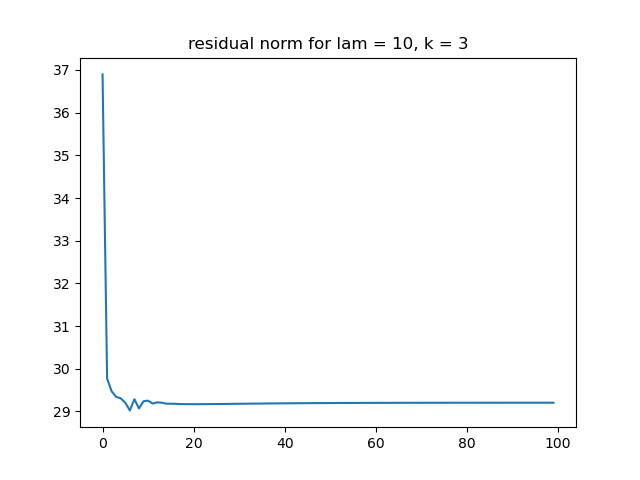
\includegraphics[scale=.3]{hw7p1 residual norm for lamcount = 3, k = 3}
			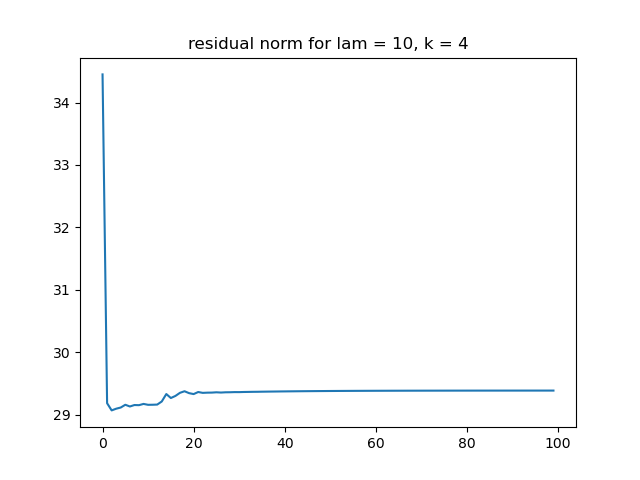
\includegraphics[scale=.3]{hw7p1 residual norm for lamcount = 3, k = 4}
			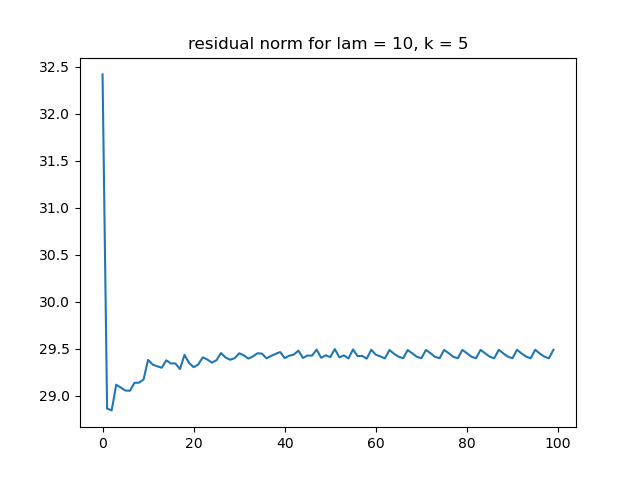
\includegraphics[scale=.3]{hw7p1 residual norm for lamcount = 3, k = 5}
			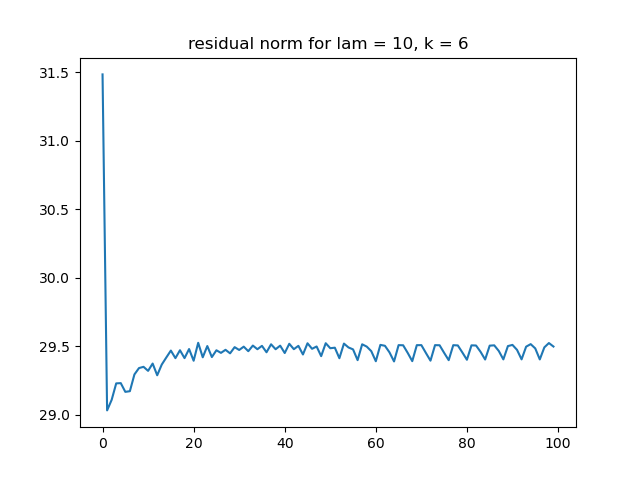
\includegraphics[scale=.3]{hw7p1 residual norm for lamcount = 3, k = 6}
			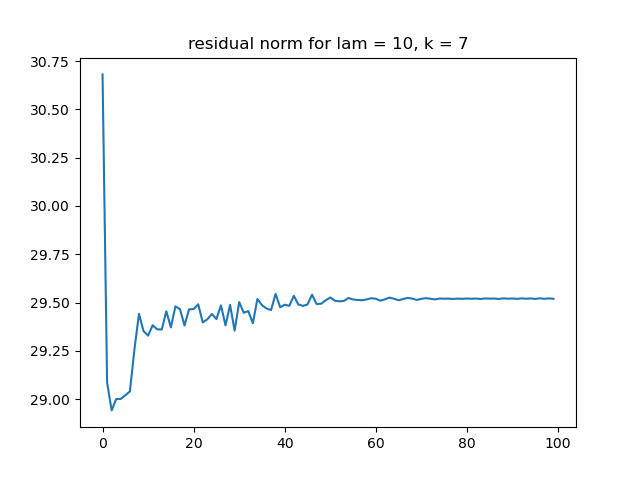
\includegraphics[scale=.3]{hw7p1 residual norm for lamcount = 3, k = 7}
		\end{center}
	
		We see that larger $k$ results in larger fluctuations in the residual norm, while larger $\lambda$ tends to dampen the fluctuations. The smallest average error between my ratings and the prediction is 0.39 which occurs at $\lambda=0.1$ and $k=6$, although there is lots of noise in the residual norm and this error is significant with respect to the rating system of 1--5.
		
		
		
		\pagebreak
		
		
		
		\item Penalizing nuclear norm:
		
		\begin{center}
			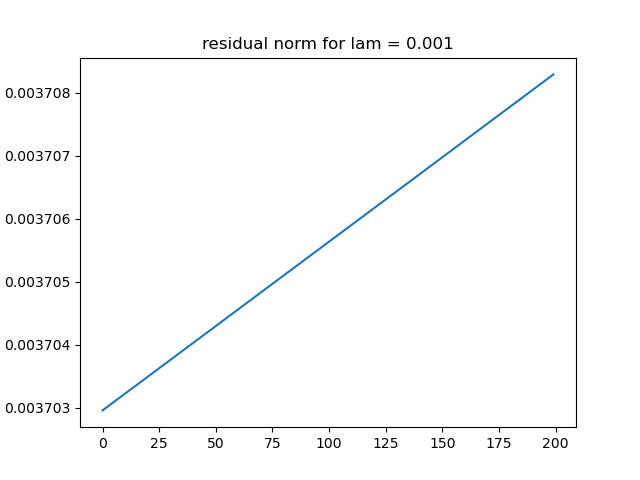
\includegraphics[scale=.3]{hw7p1b residual norm for lamcount = 1}
			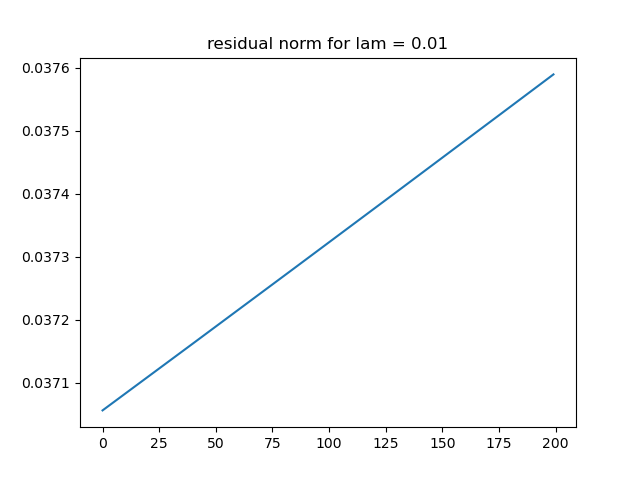
\includegraphics[scale=.3]{hw7p1b residual norm for lamcount = 2}
			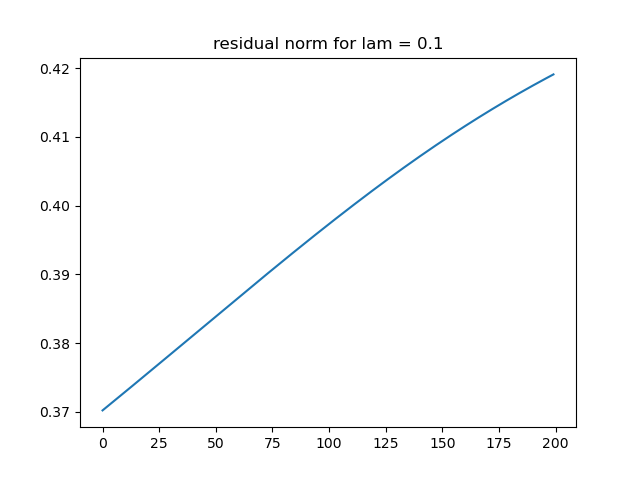
\includegraphics[scale=.3]{hw7p1b residual norm for lamcount = 3}
			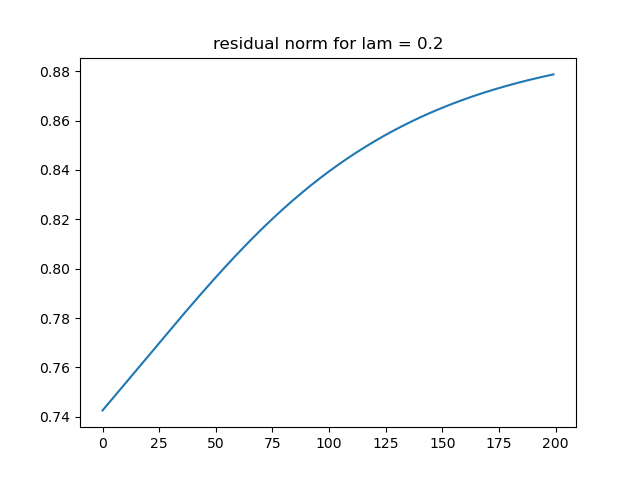
\includegraphics[scale=.3]{hw7p1b residual norm for lamcount = 4}
			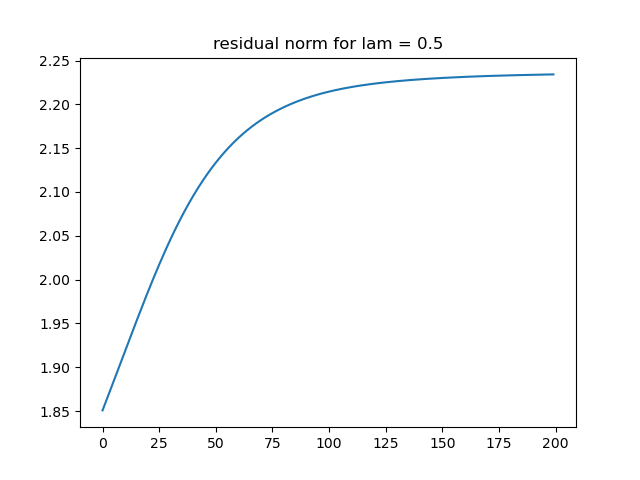
\includegraphics[scale=.3]{hw7p1b residual norm for lamcount = 5}
			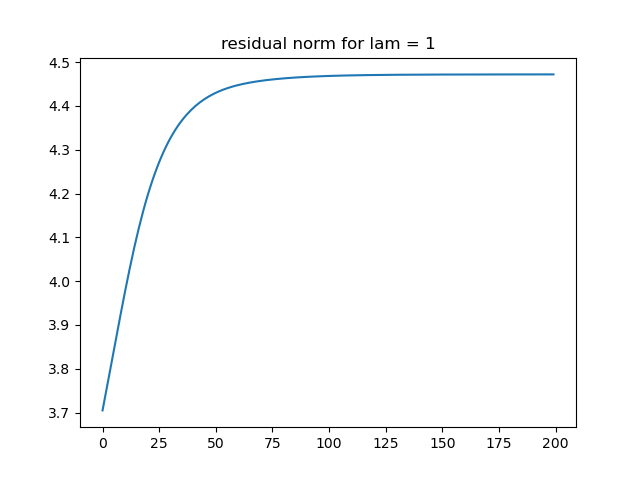
\includegraphics[scale=.3]{hw7p1b residual norm for lamcount = 6}
			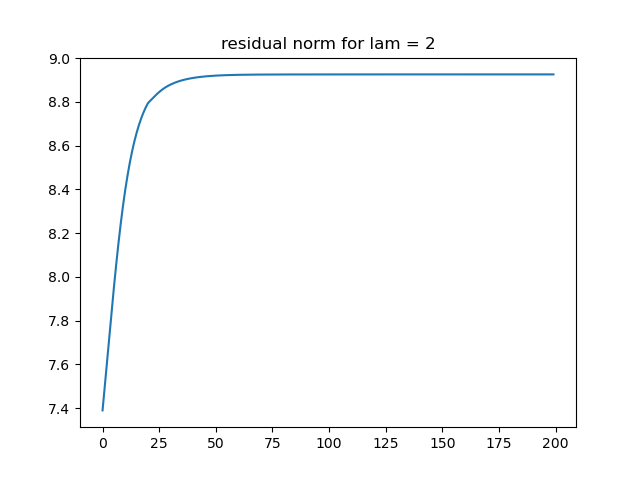
\includegraphics[scale=.3]{hw7p1b residual norm for lamcount = 7}
			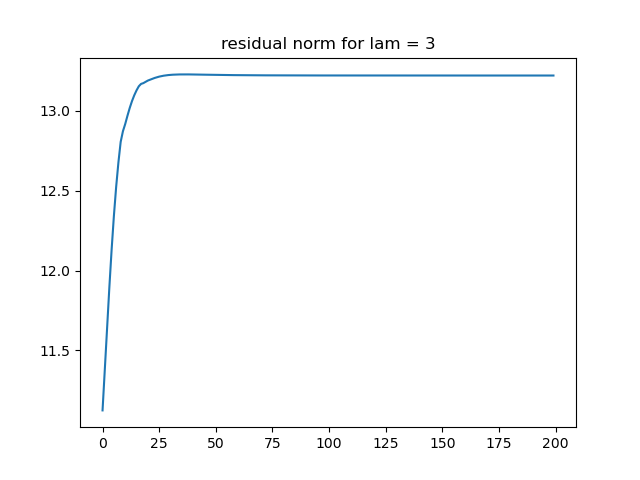
\includegraphics[scale=.3]{hw7p1b residual norm for lamcount = 8}
			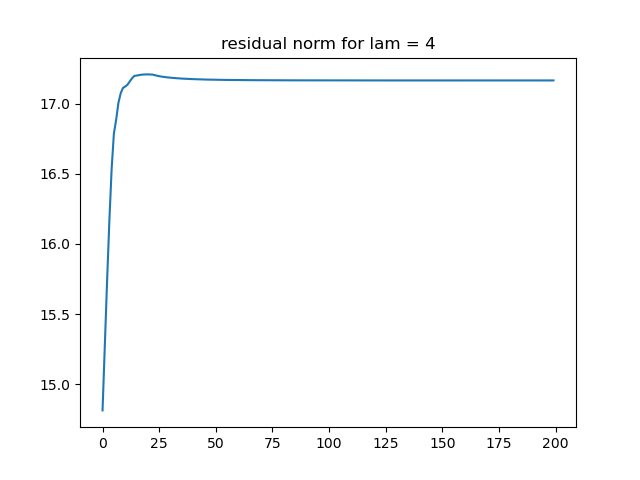
\includegraphics[scale=.3]{hw7p1b residual norm for lamcount = 9}
			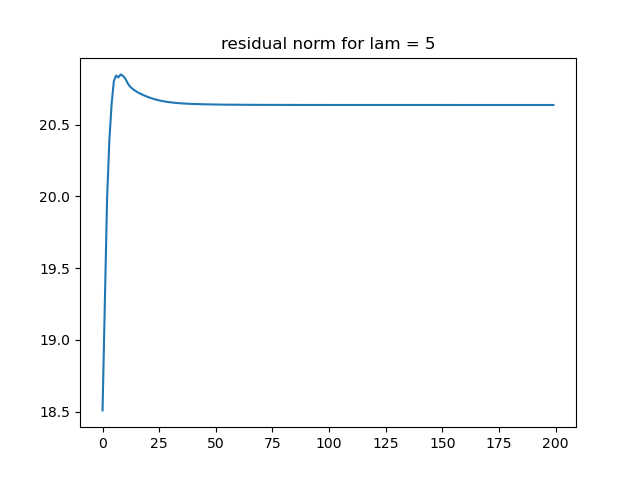
\includegraphics[scale=.3]{hw7p1b residual norm for lamcount = 10}
			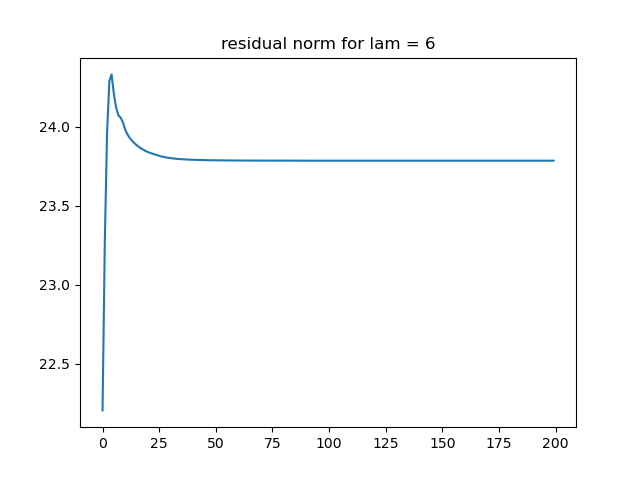
\includegraphics[scale=.3]{hw7p1b residual norm for lamcount = 11}
			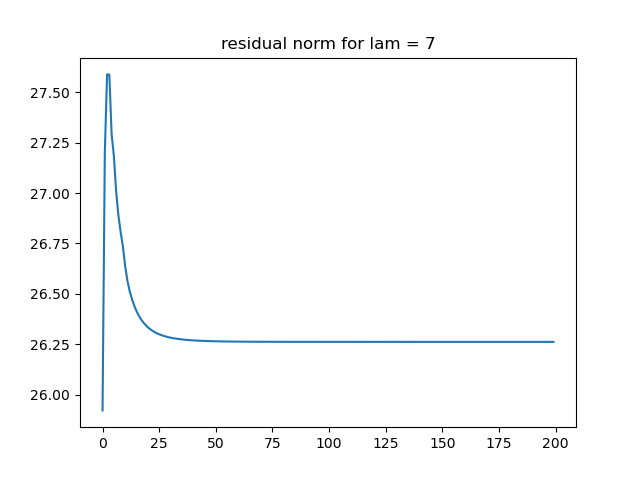
\includegraphics[scale=.3]{hw7p1b residual norm for lamcount = 12}
			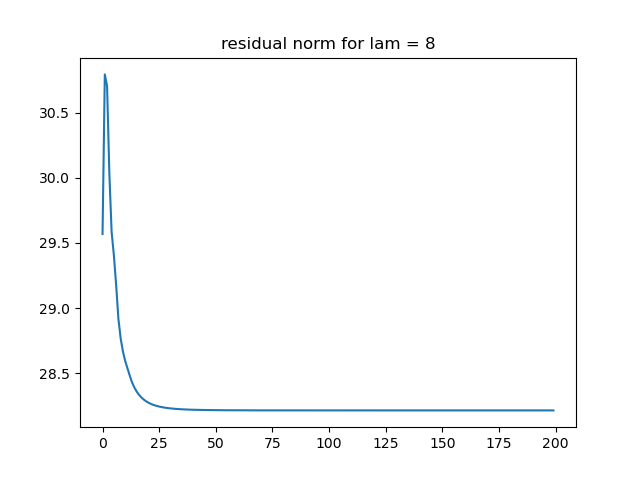
\includegraphics[scale=.3]{hw7p1b residual norm for lamcount = 13}
			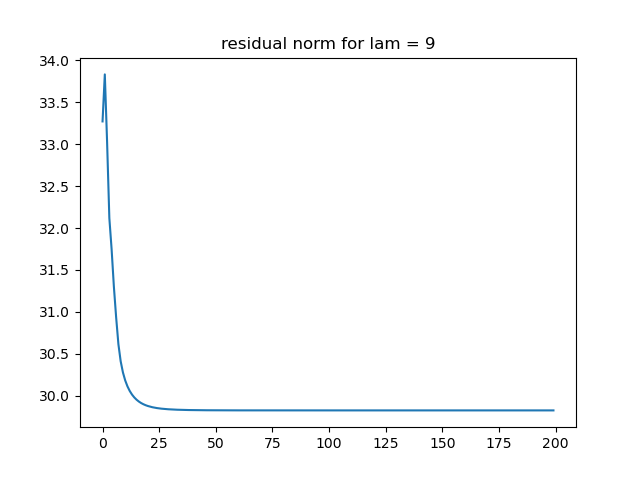
\includegraphics[scale=.3]{hw7p1b residual norm for lamcount = 14}
			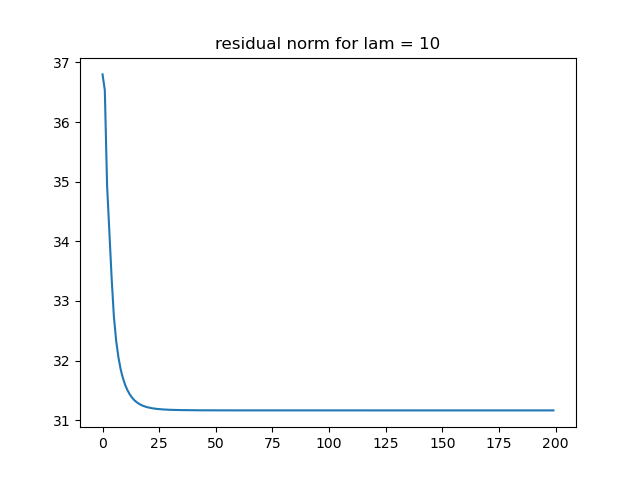
\includegraphics[scale=.3]{hw7p1b residual norm for lamcount = 15}
		\end{center}
		
		Penalizing the nuclear norm seems to give more sensible results, is easier to implement, and is faster than low rank factorization. For $\lambda=0.5$, there is a much smaller average error of 0.04 between my ratings and the prediction.
		
		
		
	\end{enumerate}
	
	
	
	\pagebreak
	
	
	
	\item Code: \url{https://github.com/RokettoJanpu/scientific-computing-1-redux/blob/main/hw7p2.ipynb}
	
	The level curve $\det A=0$ is colored red, and the level curve $\norm{A}_*=a$ is colored purple. The curves indeed intersect at the corners of $\norm{A}_*=a$.
	
	\begin{center}
		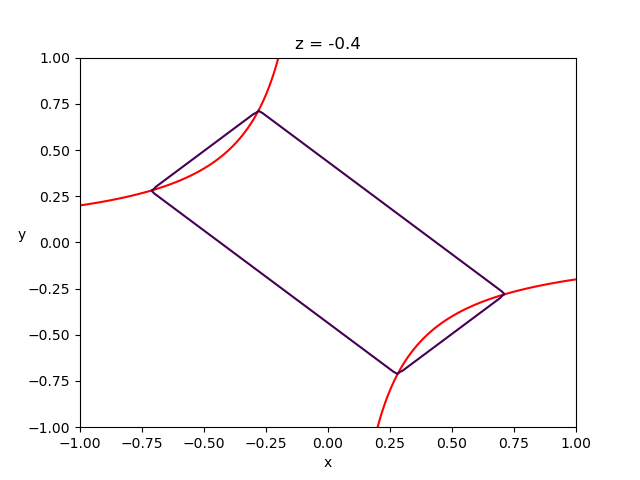
\includegraphics[scale=.3]{hw7 level curves z = -0.4}
		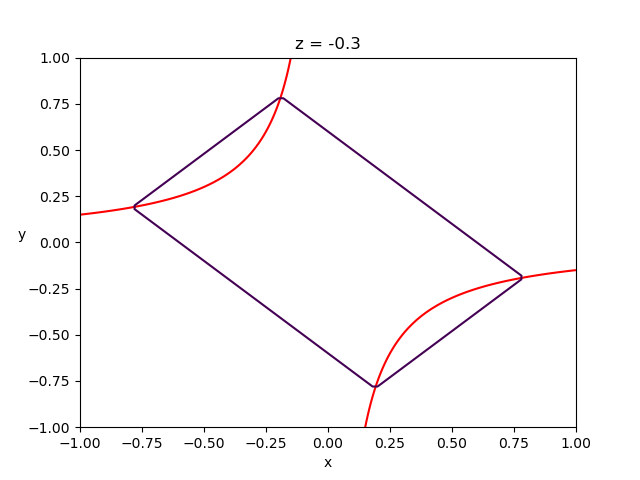
\includegraphics[scale=.3]{hw7 level curves z = -0.3}
		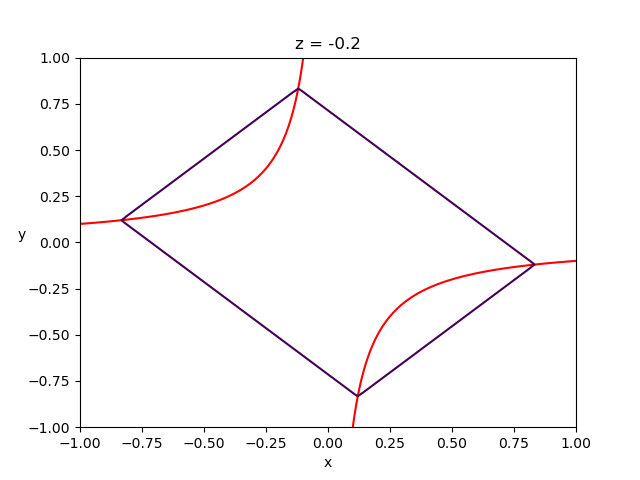
\includegraphics[scale=.3]{hw7 level curves z = -0.2}
		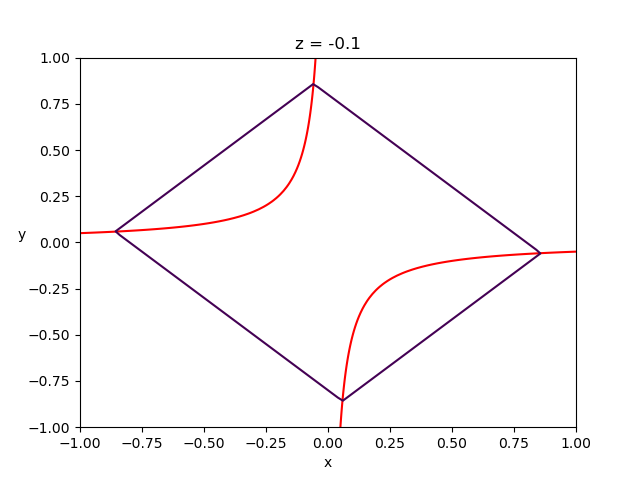
\includegraphics[scale=.3]{hw7 level curves z = -0.1}
		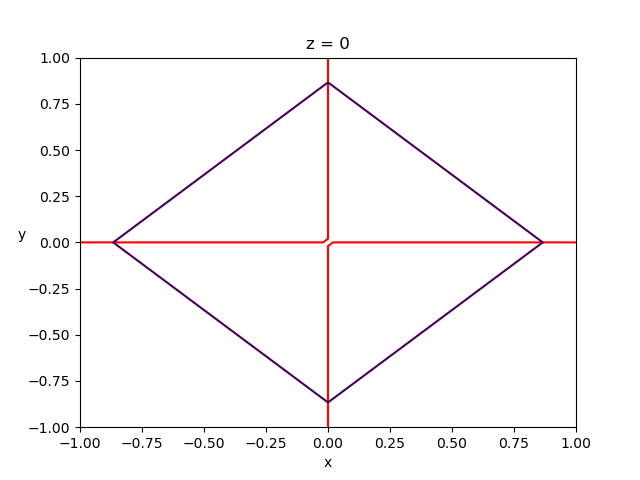
\includegraphics[scale=.3]{hw7 level curves z = 0}
		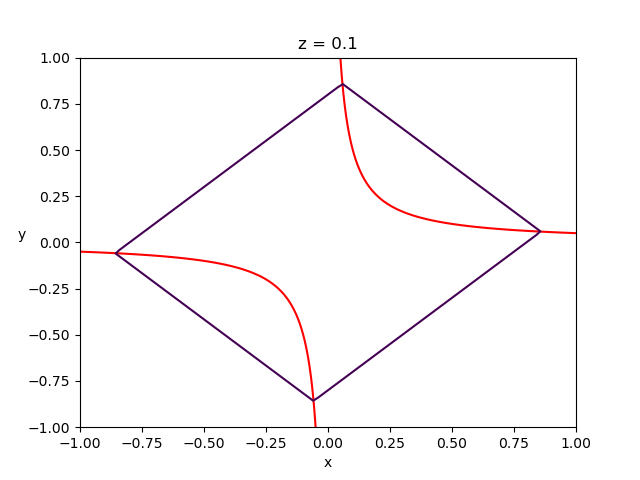
\includegraphics[scale=.3]{hw7 level curves z = 0.1}
		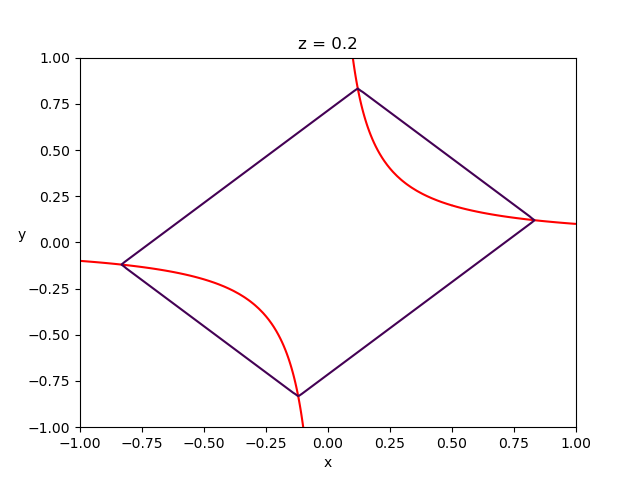
\includegraphics[scale=.3]{hw7 level curves z = 0.2}
		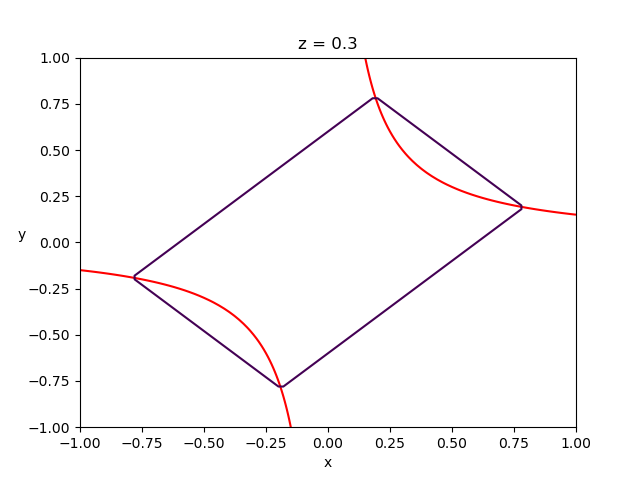
\includegraphics[scale=.3]{hw7 level curves z = 0.3}
		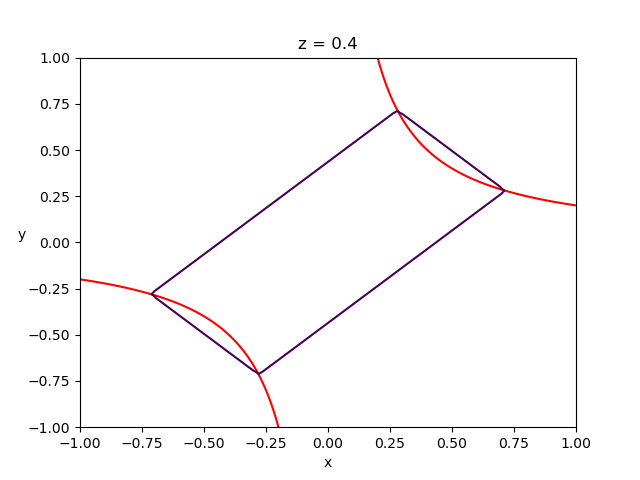
\includegraphics[scale=.3]{hw7 level curves z = 0.4}
	\end{center}
	
	
	
	\pagebreak
	
	
	
	\item We will use the "direct" definition of linear independence. Let $c_0,\dots,c_{n-1}\in\bR$ satisfy
	\[\sum_{k=0}^{n-1}c_kp_k = 0\]
	Left multiply both sides by $A$.
	\[\sum_{k=0}^{n-1}c_kAp_k = 0\]
	Fix $j$ and left multply both sides by $p_j^T$. Since $p_j^TAp_k=0$ for all $k\ne j$,
	\[c_jp_j^TAp_j = 0\]
	Since $A$ is SPD and $p_j\ne0$, we have $p_j^TAp_j>0$, hence $c_j=0$.
	
	
	
\end{enumerate}
	
	
	
\end{document}